% !TeX spellcheck = en_GB
\ifcsname SlidesDistr\endcsname%
	\documentclass[handout,aspectratio=169]{beamer}
\else%
	\documentclass[aspectratio=169]{beamer}
\fi%
\usepackage{fontspec}
\usepackage[T1]{fontenc}
\usepackage{amsmath}
\usepackage{amsfonts}
\usepackage{amssymb}
\usepackage{graphicx}
\usepackage{csquotes}
\usepackage{booktabs}
\usepackage{multicol}
\usepackage{enumerate}
\usepackage{microtype}
\usepackage[labelfont=bf,font={small}]{caption}
\usepackage{hyperref}
\usepackage{booktabs}
\usepackage{subcaption}
\usepackage{fancyhdr}
\usepackage{pdfpages}
\usepackage{siunitx}
\usepackage{tikz}
\usepackage{mdframed}

\defaultfontfeatures{Mapping=tex-text}
\newfontfamily\symbolfont{Symbola}
\newfontfamily\quotefont{GentiumPlus}

\usepackage[sorting=none]{biblatex}
\addbibresource{../bibliography.bib}

\author{Chris Eliasmith}


\renewcommand{\vec}[1]{{\mathbf{#1}}}
\newcommand{\mat}[1]{{\mathbf{#1}}}
\newcommand{\T}{\ensuremath{\mathsf{T}}}
\renewcommand{\epsilon}{\varepsilon}
\renewcommand{\phi}{\varphi}

% Tango color palette
\definecolor{butter1}{HTML}{FCE94F}
\definecolor{butter2}{HTML}{EDD400}
\definecolor{butter3}{HTML}{C4A000}
\definecolor{orange1}{HTML}{FCAF3E}
\definecolor{orange2}{HTML}{F57900}
\definecolor{orange3}{HTML}{CE5C00}
\definecolor{chocolate1}{HTML}{E9B96E}
\definecolor{chocolate2}{HTML}{C17D11}
\definecolor{chocolate3}{HTML}{8F5902}
\definecolor{chameleon1}{HTML}{8AE234}
\definecolor{chameleon2}{HTML}{73D216}
\definecolor{chameleon3}{HTML}{4E9A06}
\definecolor{skyblue1}{HTML}{729FCF}
\definecolor{skyblue2}{HTML}{3465A4}
\definecolor{skyblue3}{HTML}{204A87}
\definecolor{plum1}{HTML}{AD7FA8}
\definecolor{plum2}{HTML}{75507B}
\definecolor{plum3}{HTML}{5C3566}
\definecolor{scarletred1}{HTML}{EF2929}
\definecolor{scarletred2}{HTML}{CC0000}
\definecolor{scarletred3}{HTML}{A40000}
\definecolor{aluminium1}{HTML}{EEEEEC}
\definecolor{aluminium2}{HTML}{D3D7CF}
\definecolor{aluminium3}{HTML}{BABDB6}
\definecolor{aluminium4}{HTML}{888A85}
\definecolor{aluminium5}{HTML}{555753}
\definecolor{aluminium6}{HTML}{2E3436}

\definecolor{violet}{HTML}{AA305C}
\definecolor{uwyellow}{HTML}{FDD433}
\definecolor{background}{HTML}{F9F9F6}
\definecolor{text}{HTML}{000000}

\definecolor{uweng1}{HTML}{D1B2EE}
\definecolor{uweng2}{HTML}{BF33DE}
\definecolor{uweng3}{HTML}{8001B3}
\definecolor{uweng4}{HTML}{56048A}

\setbeamercolor{title}{fg=violet}
\setbeamercolor{frametitle}{fg=black}
\setbeamercolor{structure}{fg=aluminium5}
\setbeamercolor{normal text}{fg=text}

\setbeamertemplate{navigation symbols}{}
\setbeamertemplate{footline}[frame number]

\hypersetup{%
	colorlinks=false,% hyperlinks will be black
	urlbordercolor=aluminium4,% hyperlink borders will be red
	pdfborderstyle={/S/U/W 0.5}% border style will be underline of width 1pt
}

\makeatletter
\newcommand{\superimpose}[2]{%
	{\ooalign{{#1}\hidewidth\cr{#2}\hidewidth\cr}}}
\makeatother
\newcommand{\SolidCircle}[2]{\superimpose{\color{#1}\symbolfont ⬤}{\textbf{\color{white}#2}}\hspace{1em}}
\newcommand{\OPlus}{\SolidCircle{chameleon3}{\kern0.75pt+}}
\newcommand{\OMeh}{\SolidCircle{uwyellow}{~}}
\newcommand{\OMinus}{\SolidCircle{scarletred3}{\kern2.25pt--}}

\newcommand{\hl}[1]{\colorbox{uwyellow}{{\color{black}\textbf{#1}}}}

\newcommand{\ImageSources}[1]{%
	\begin{columns}%
		\column{1.1\textwidth}%
		\raggedright%
		\tiny\color{aluminium4}%
		\setlength\lineskip{1em}%
		\textbf{Image Sources.}	{#1}%
	\end{columns}}

\newcommand{\ColorRect}[3]{{\color{#1}\rule{#2}{#3}}}
\setbeamertemplate{headline}{\ColorRect{black}{\textwidth}{4pt}\newline\ColorRect{uweng1}{0.25\textwidth}{4pt}\ColorRect{uweng2}{0.25\textwidth}{4pt}\ColorRect{uweng3}{0.25\textwidth}{4pt}\ColorRect{uweng4}{0.25\textwidth}{4pt}}

\newcommand{\MakeTitle}{%
	\vspace{0.5cm}%
	{\textbf{\inserttitle}}\\[0.5cm]%
	\insertauthor\\[0.5cm]%
	\insertdate\\%
	\begin{itemize}
		\item Slide design: Andreas Stöckel
		\item Content: Terry Stewart, Andreas Stöckel, Chris Eliasmith
	\end{itemize}
 	
\includegraphics[width=7cm]{../assets/uwlogo_eng.pdf}%
}

\newcommand{\handwritingframe}{%
	\begin{frame}
		\begin{columns}
			\column{\paperwidth}
			
\includegraphics{../assets/handwriting_lines.pdf}
		\end{columns}
	\end{frame}	
}

\newcommand{\imageframe}[1]{%
	\setbeamertemplate{navigation symbols}{}%
	\begin{frame}[plain,noframenumbering]%
		\begin{tikzpicture}[remember picture,overlay]%
		\node[at=(current page.center)] {%
			\includegraphics[width=\paperwidth]{#1}%
		};%
		\end{tikzpicture}%
	\end{frame}%
}

\newcommand{\videoframe}[3][mp4]{%
	\begin{frame}[plain,noframenumbering]%
		\hypersetup{%
			pdfborderstyle={/S/U/W 0}% border style will be underline of width 1pt
		}%
		\begin{tikzpicture}[remember picture,overlay]%
		\node[at=(current page.center)] {%
			\includegraphics[width=\paperwidth]{{video/#2_#3}.jpg}%
		};%
		\node[at=(current page.center)] {%
			\ifcsname SlidesDistr\endcsname%
				\href{https://youtu.be/#3}{
\includegraphics[width=2cm]{../assets/play_button.pdf}}%
			\else%
				\href{video/#2_#3.#1}{
\includegraphics[width=2cm]{../assets/play_button.pdf}}%
			\fi%
		};%
		\end{tikzpicture}%
	\end{frame}%
}

\newcommand{\includevideo}[4][mp4]{%
	\begingroup%
	\hypersetup{%
		pdfborderstyle={/S/U/W 0}% border style will be underline of width 1pt
	}%
	\begin{tikzpicture}%
	\node (A) {%
		\includegraphics[width=#4]{{video/#2_#3}.jpg}%
	};%
	\node[at=(A.center)] {%
		\ifcsname SlidesDistr\endcsname%
			\href{https://youtu.be/#3}{
\includegraphics[width=2cm]{../assets/play_button.pdf}}%
		\else%
			\href{video/#2_#3.#1}{
\includegraphics[width=2cm]{../assets/play_button.pdf}}%
		\fi%
	};%
	\end{tikzpicture}%
	\endgroup%
}

\newcommand{\backupbegin}{
	\newcounter{finalframe}
	\setcounter{finalframe}{\value{framenumber}}
	\setbeamertemplate{footline}{}
}

\newcommand{\backupend}{
	\setcounter{framenumber}{\value{finalframe}}
}


\date{Sept 20 \& 25, 2023}
\title{SYDE 556/750 \\ Simulating Neurobiological Systems \\ Lecture 4: Temporal Representations}

\begin{document}

\begin{frame}{}
	\vspace{0.5cm}
	\begin{columns}[c]
		\column{0.6\textwidth}
		\MakeTitle
		\column{0.4\textwidth}
		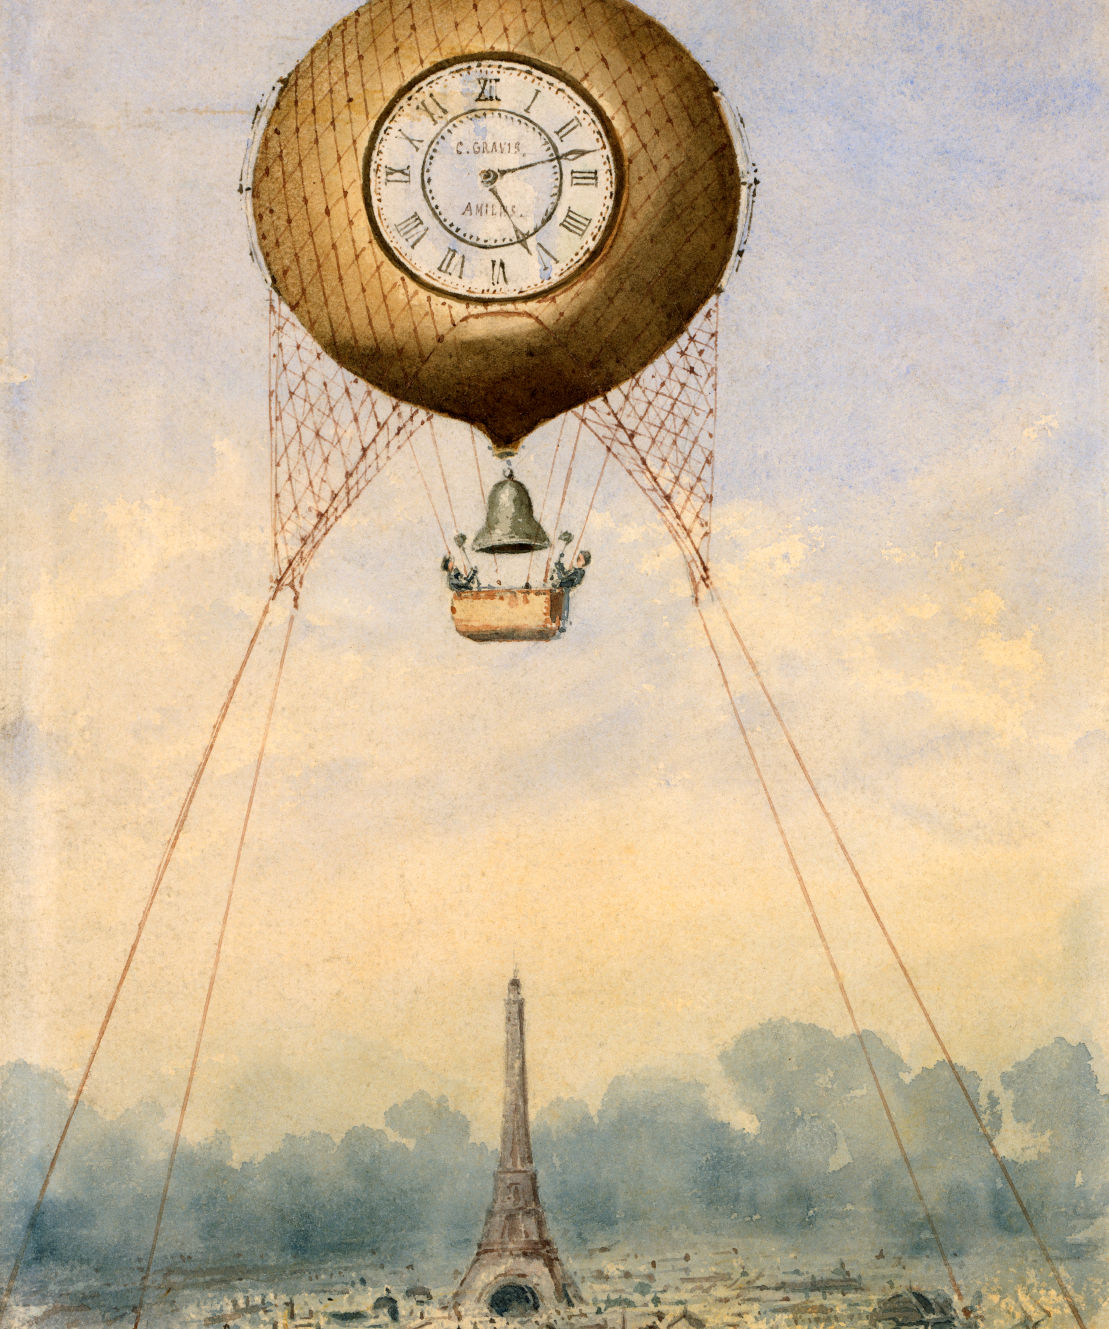
\includegraphics[width=\textwidth]{media/camille_gravis_captive_balloon_with_clock_face_small.jpg}
	\end{columns}
\end{frame}

\begin{frame}{Reminder: The LIF Neuron}
	\begin{columns}[c]
		\column{0.6\textwidth}
		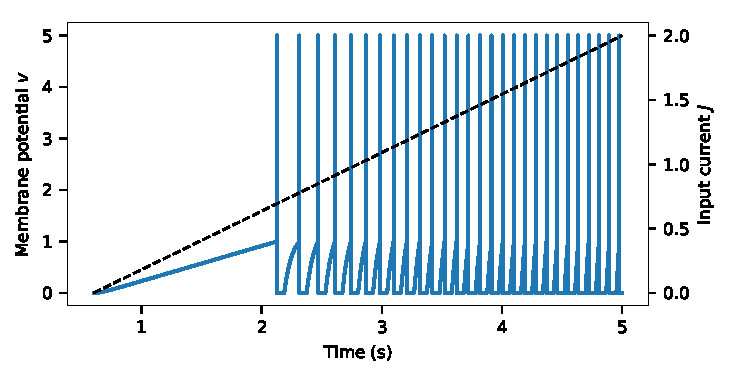
\includegraphics[width=\textwidth]{media/lif_neuron_ramp.pdf}
		\column{0.4\textwidth}
		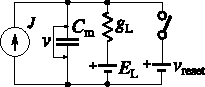
\includegraphics[width=\textwidth]{media/lif_circuit.pdf}
	\end{columns}
	\begin{align*}
		\frac{\mathrm{d}}{\mathrm{d}t} v(t) &= -\frac{1}{\tau_\mathrm{RC}} \big( v(t) - J \big) \,, \quad &\text{if } v(t) &< 1\,, \\
		v(t) &\gets \delta(t - t_\mathrm{th}) \,, &\text{if } t &= t_\mathrm{th} \,,\\
		v(t) &\gets 0 \,, &\text{if } t &> t_\mathrm{th} \text{ and } t \geq t_\mathrm{th} + \tau_\mathrm{ref} \,,
	\end{align*}
\end{frame}

\begin{frame}{Temporal Decoding of Two Neurons - Weighted Spikes}
	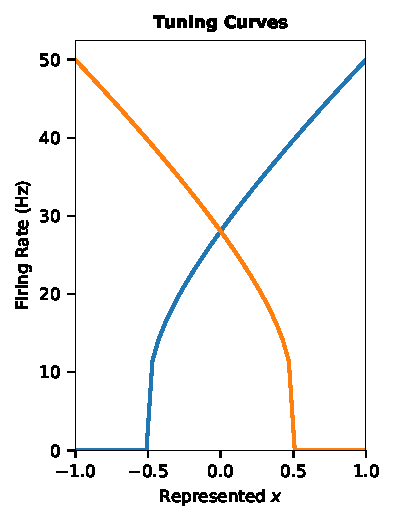
\includegraphics[width=0.4\textwidth]{media/two_neurons_tuning_curves.pdf}%
	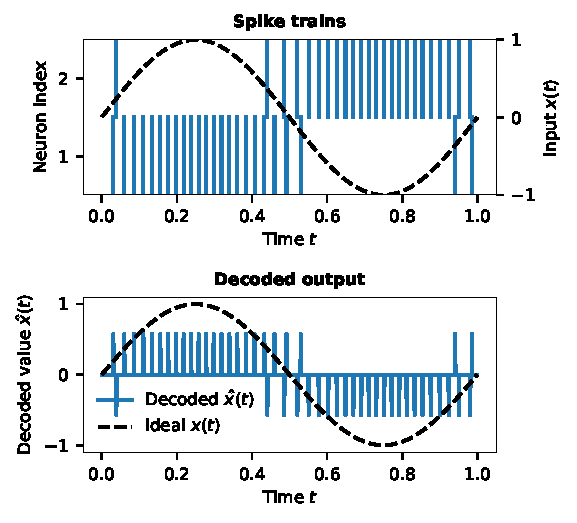
\includegraphics[width=0.6\textwidth]{media/two_neurons_spike_train.pdf}
\end{frame}

\begin{frame}{Temporal Decoding of One Hundred Neurons - Weighted Spikes}
	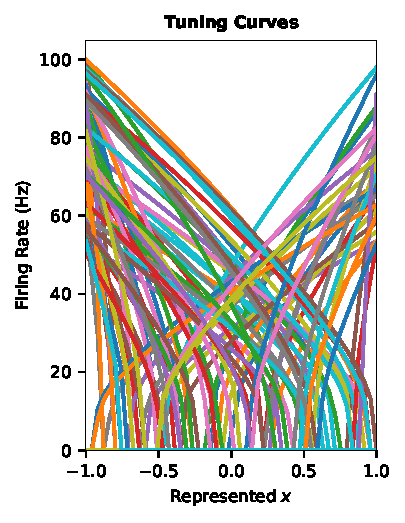
\includegraphics[width=0.4\textwidth]{media/hundred_neurons_tuning_curves.pdf}%
	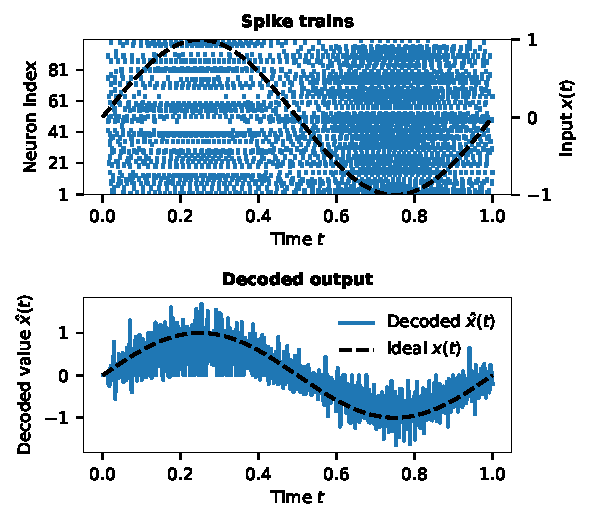
\includegraphics[width=0.6\textwidth]{media/hundred_neurons_spike_train.pdf}
\end{frame}

\begin{frame}{Random Signals}
	\begin{overlayarea}{\textwidth}{0.9\textheight}
		\begin{columns}
			\column{0.75\textwidth}
			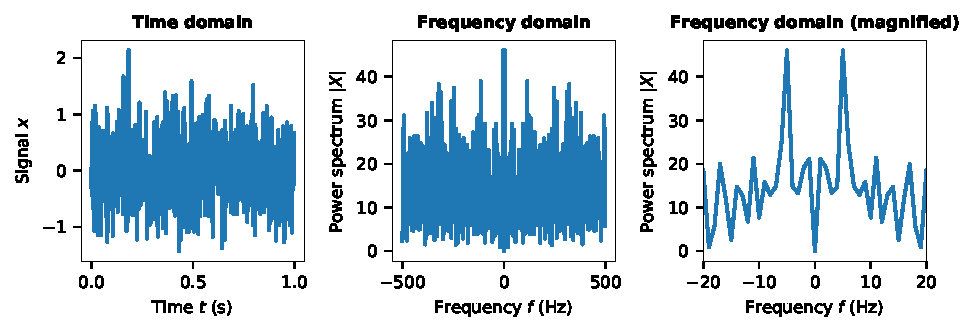
\includegraphics[width=\textwidth]{media/white_noise.pdf}
			\column{0.25\textwidth}
			\hl{White Noise}\\
			(zero mean)
		\end{columns}
		\only<2>{\begin{columns}
			\column{0.75\textwidth}
			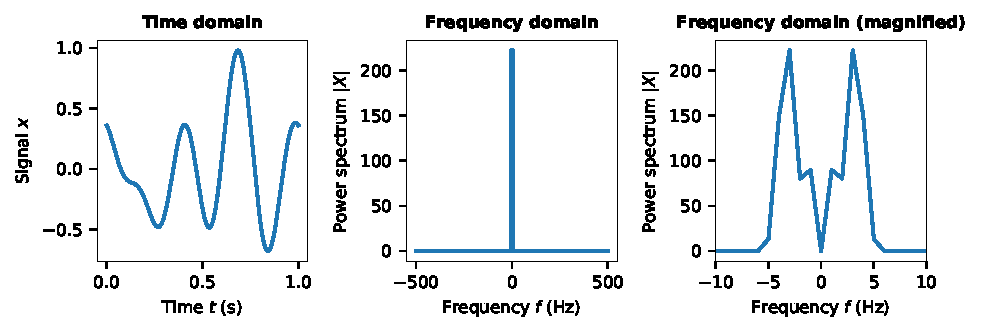
\includegraphics[width=\textwidth]{media/white_noise_5hz.pdf}
			\column{0.25\textwidth}
			\hl{Bandlimited}\\White Noise\\
			(zero mean,\\\SI{5}{\hertz} bandwidth)
		\end{columns}}
		\only<3>{\begin{columns}
			\column{0.75\textwidth}
			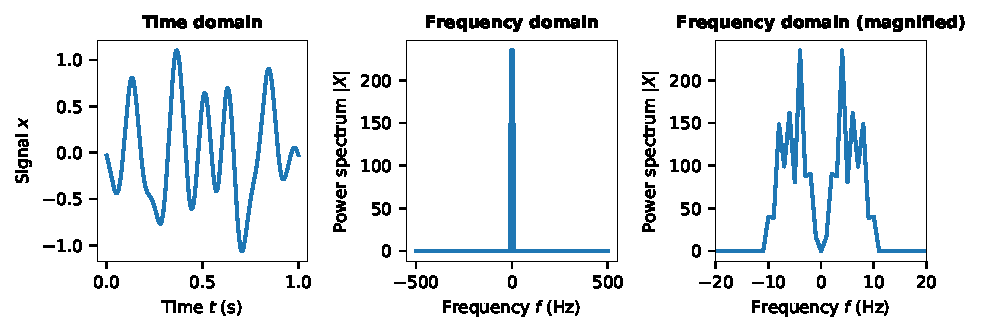
\includegraphics[width=\textwidth]{media/white_noise_10hz.pdf}
			\column{0.25\textwidth}
			\hl{Bandlimited}\\White Noise\\
			(zero mean,\\\SI{10}{\hertz} bandwidth)
			\end{columns}}
	\end{overlayarea}
\end{frame}

\begin{frame}{Filtering by Convolution}
	\begin{columns}
		\column{0.5\textwidth}
		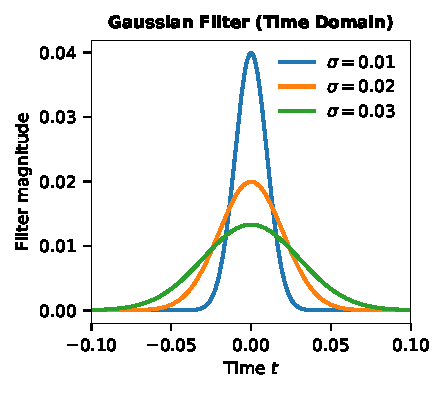
\includegraphics[width=\textwidth]{media/gaussian_filters.pdf}
		\column{0.5\textwidth}
		\begin{block}{Gaussian Filter}
			\begin{align*}
				h(t) &= c \exp \left( \frac{-t^2}{\sigma^2} \right) \\
				\text{where }  &~c \text{ chosen s.t. } {\textstyle \int_{-\infty}^\infty h(t) \,\mathrm{d}t = 1}
			\end{align*}
		\end{block}
		\begin{block}{Convolution}
			\begin{align*}
				\big( f \ast h \big)(t) &= \int_{-\infty}^{\infty} f(t - t') h(t') \,\mathrm{d}t'
			\end{align*}
		\end{block}
	\end{columns}
\end{frame}

\begin{frame}{Filtering a Spike Train}
	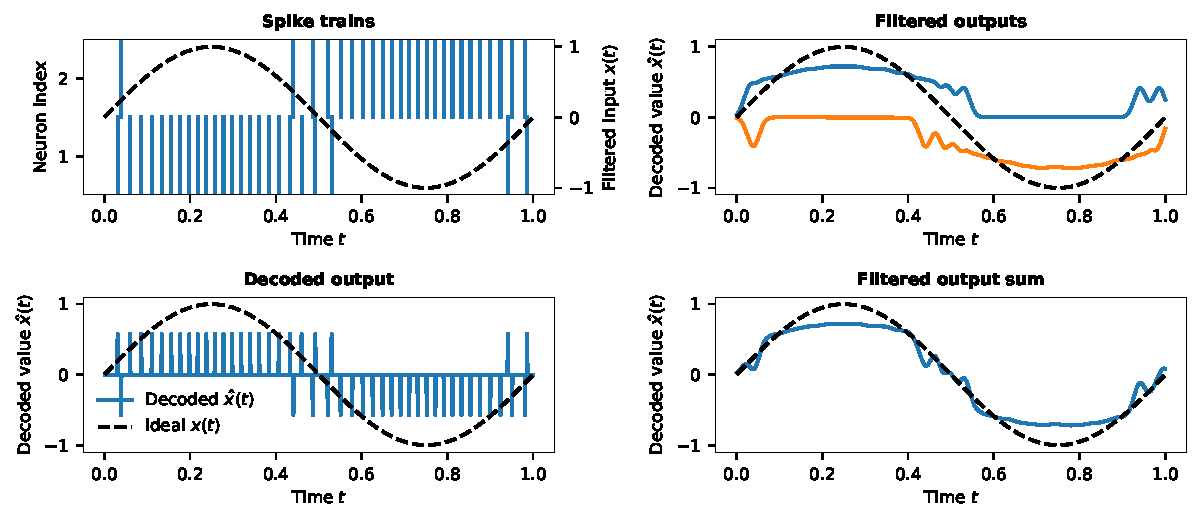
\includegraphics[width=\textwidth]{media/two_neurons_filtered.pdf}
\end{frame}

\begin{frame}{Filtering a Spike Train for a Random Signal}
	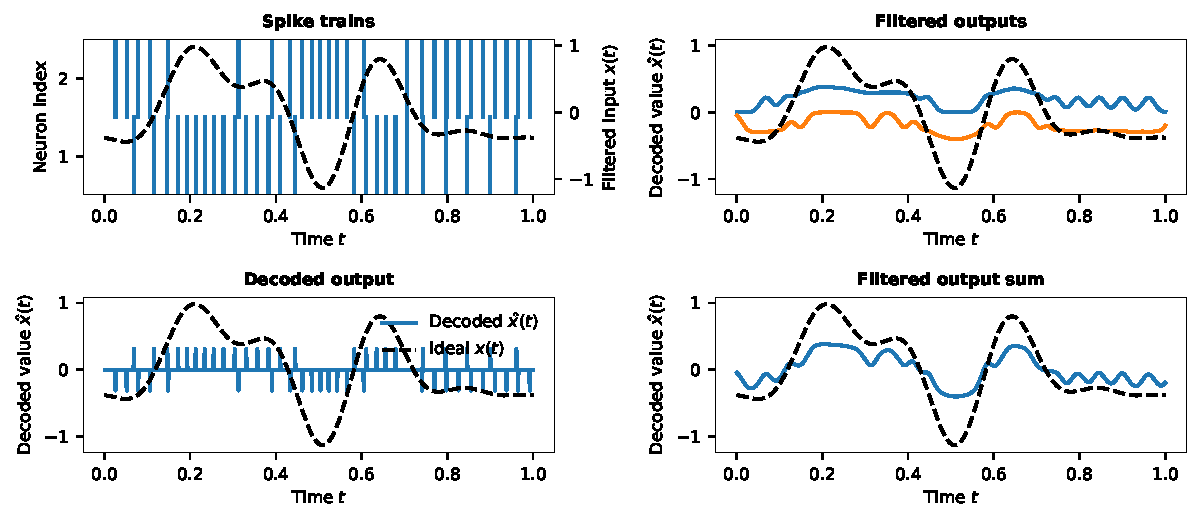
\includegraphics[width=\textwidth]{media/two_neurons_filtered_white_noise.pdf}
\end{frame}

\begin{frame}{Optimal Filter}
	\centering
	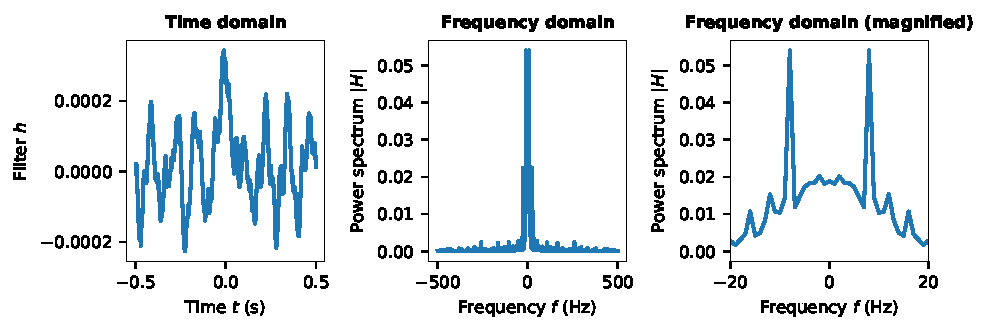
\includegraphics[width=\textwidth]{media/optimal_filter.pdf}\\
	$$H(\omega) = {{X(\omega) \overline{R}(\omega)} \over {|R(\omega)|^2}}$$
\end{frame}

\begin{frame}{Filtering a Spike Train for a Random Signal (Optimal Filter)}
	\includegraphics<1>[width=\textwidth]{media/two_neurons_filtered_white_noise.pdf}
	\includegraphics<2>[width=\textwidth]{media/two_neurons_filtered_optimal_simple.pdf}
	\includegraphics<3>[width=\textwidth]{media/two_neurons_filtered_optimal_simple_2.pdf}
	\includegraphics<4>[width=\textwidth]{media/two_neurons_filtered_optimal_simple_3.pdf}
\end{frame}

\begin{frame}{Optimal Filter (Improved)}
	\centering
	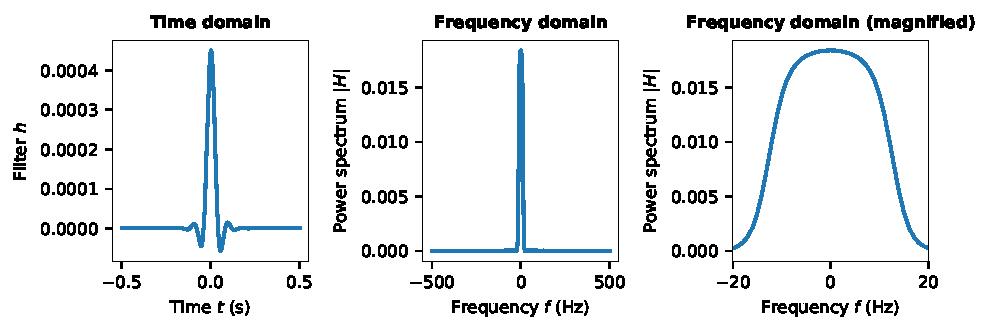
\includegraphics[width=\textwidth]{media/optimal_filter_improved.pdf}\\
	$$H(\omega) = {{X(\omega) \overline{R}(\omega)} \ast W(\omega) \over {|R(\omega)|^2} \ast W(\omega)} $$
\end{frame}

\begin{frame}{Filtering a Spike Train for a Random Signal (Improved Optimal Filter)}
	\includegraphics<1>[width=\textwidth]{media/two_neurons_filtered_optimal_simple.pdf}
	\includegraphics<2>[width=\textwidth]{media/two_neurons_filtered_optimal.pdf}
	\includegraphics<3>[width=\textwidth]{media/two_neurons_filtered_optimal_2.pdf}
	\includegraphics<4>[width=\textwidth]{media/two_neurons_filtered_optimal_3.pdf}
\end{frame}

\begin{frame}{Pros and Cons of the Optimal Filter}
	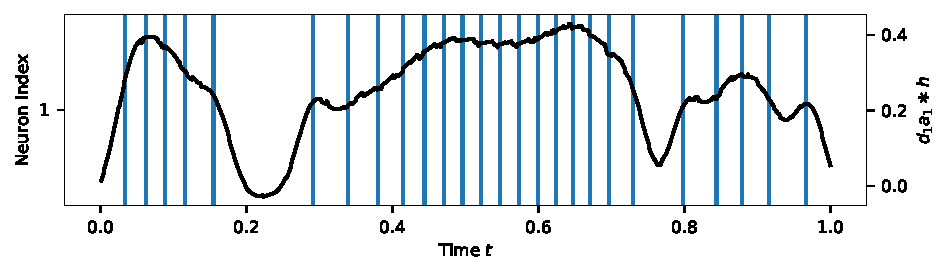
\includegraphics[width=\textwidth]{media/filter_magnification.pdf}
	\begin{columns}[t]
		\column{0.5\textwidth}
		\begin{itemize}
			\item<2->[\OPlus] \textbf{Precise}\\Good for analysing data after the fact
		\end{itemize}
		\column{0.5\textwidth}
		\begin{itemize}
			\item<3->[\OMinus] \hl{Non-causal}\\Does not describe a biological process
		\end{itemize}
	\end{columns}
	\vspace{0.5cm}
	\begin{overlayarea}{\textwidth}{0.5cm}
		\centering
		\quotefont\large
		\only<4->{We need to find a mechanism that low-pass filters spikes over time!}
	\end{overlayarea}
\end{frame}

\begin{frame}{Synapses as Filters}
	\centering
	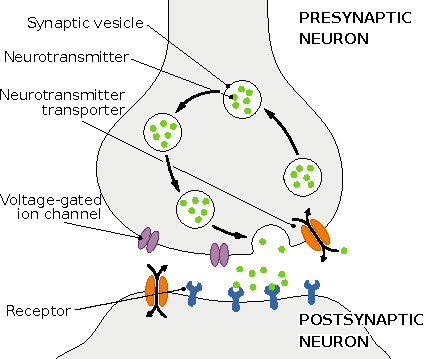
\includegraphics[width=0.375\textwidth]{media/synapse_schematic.pdf}~~%
	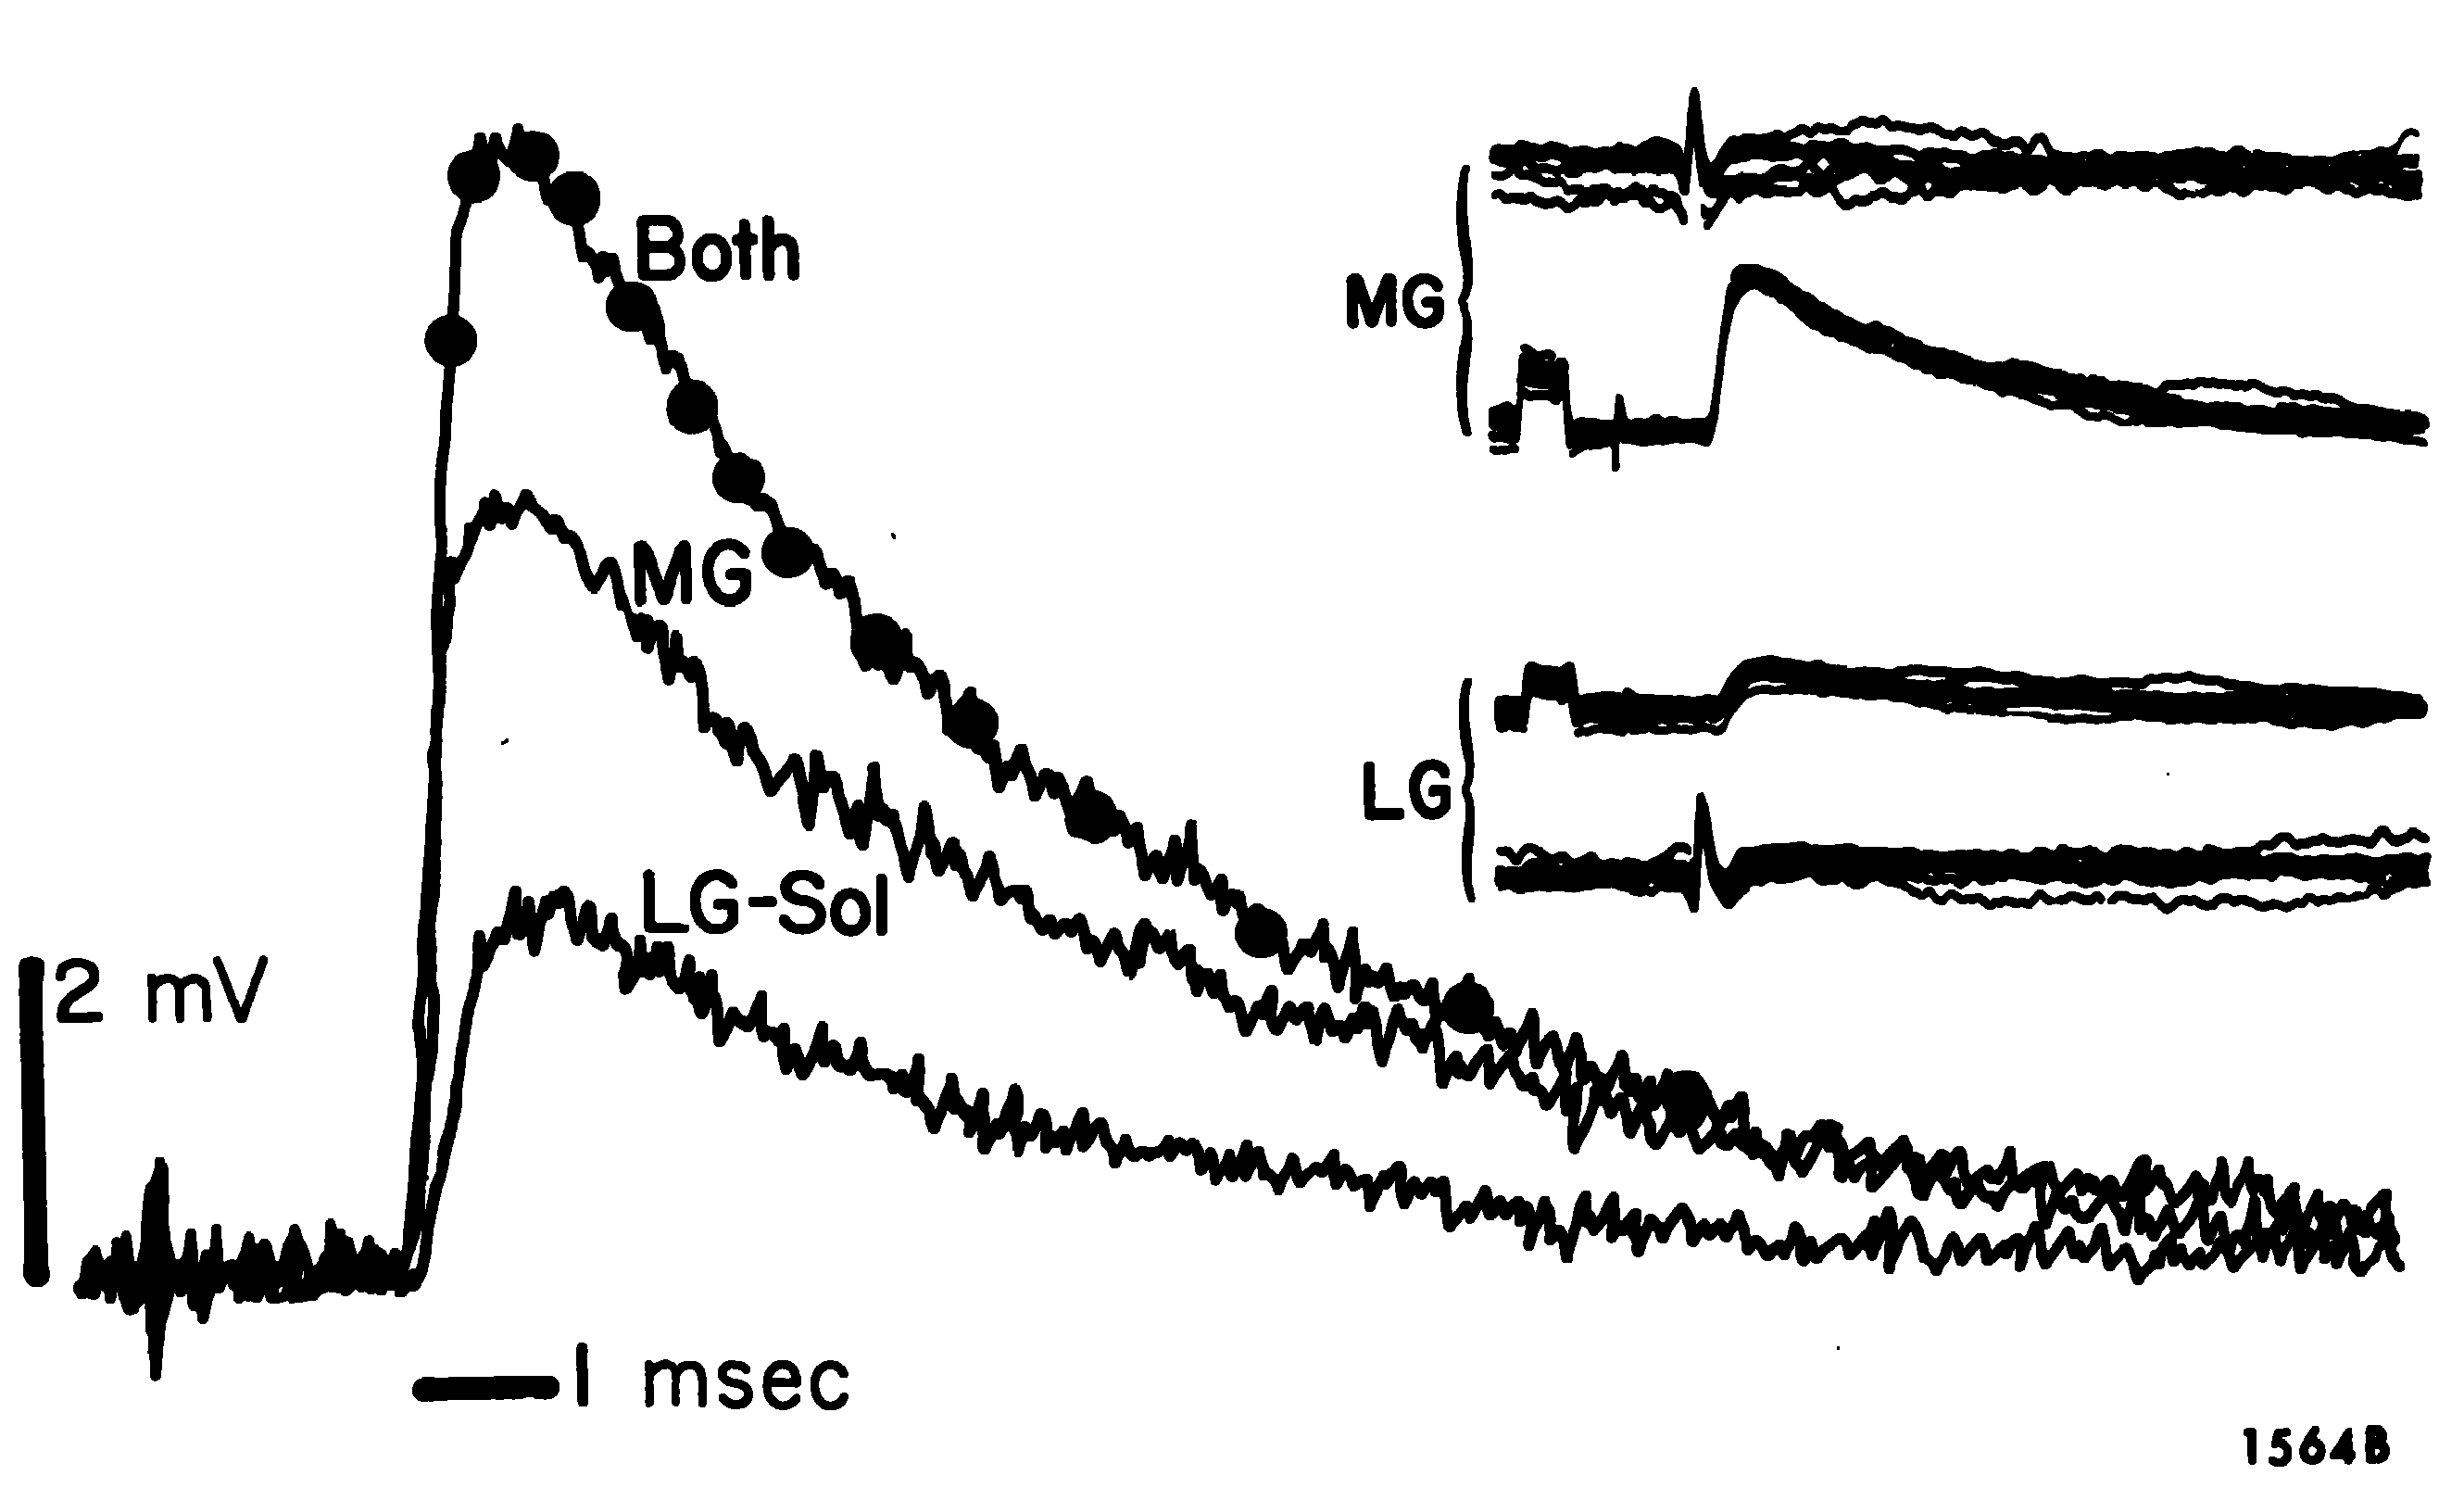
\includegraphics[width=0.55\textwidth]{media/burke_1967_epsp.png}\\[0.5cm]
	\centering
	\begin{overlayarea}{\textwidth}{0.5cm}
		\centering
		\only<2->{\quotefont\large
		\hl{Post-synaptic currents (EPSCs, IPSCs) are low-pass filtered spike trains!}}
	\end{overlayarea}
\end{frame}

\begin{frame}{Exponential Low-Pass Filter (I)}
	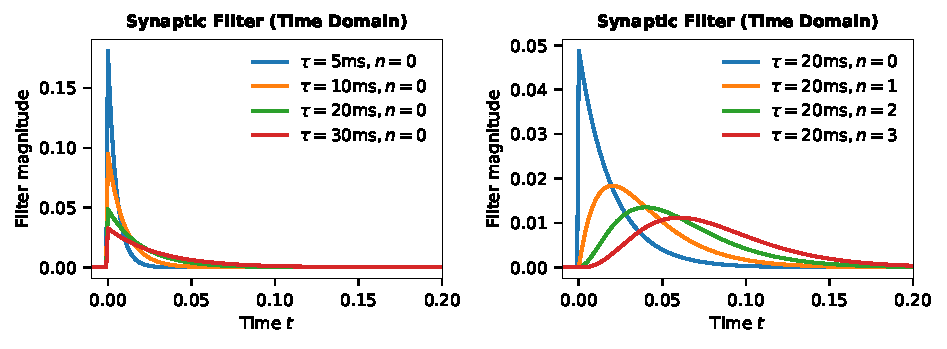
\includegraphics[width=\textwidth]{media/synaptic_filters.pdf}
	\begin{align*}
			h(t) &= \begin{cases}
		c^{-1} t^n \exp^{-t / \tau} & \text{if } t \geq 0 \,,\\
		0 & \text{otherwise}\,,
		\end{cases}
		&& \text{where } c = \int_{0}^\infty t^n \exp^{-t / \tau} \,\mathrm{d}t \,.
	\end{align*}
\end{frame}

\begin{frame}{Exponential Low-Pass Filter (II)}
	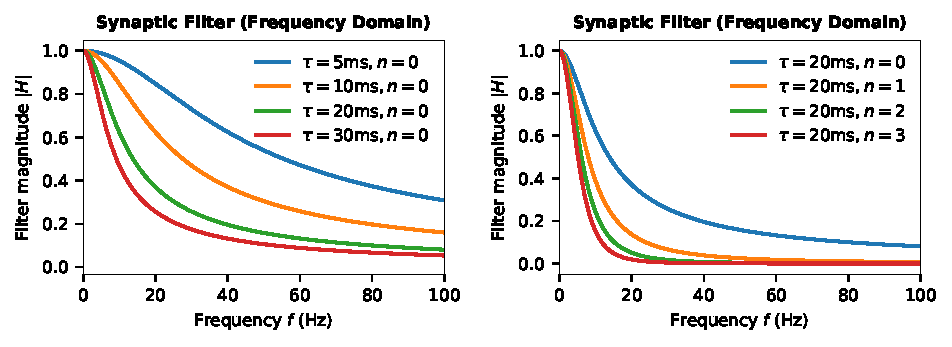
\includegraphics[width=\textwidth]{media/synaptic_filters_freq.pdf}
	\begin{align*}
	h(t) &= \begin{cases}
	c^{-1} t^n \exp^{-t / \tau} & \text{if } t \geq 0 \,,\\
	0 & \text{otherwise}\,,
	\end{cases}
	&& \text{where } c = \int_{0}^\infty t^n \exp^{-t / \tau} \,\mathrm{d}t \,.
	\end{align*}
\end{frame}

\begin{frame}{Example: Synaptic Filter for Two Neurons}
	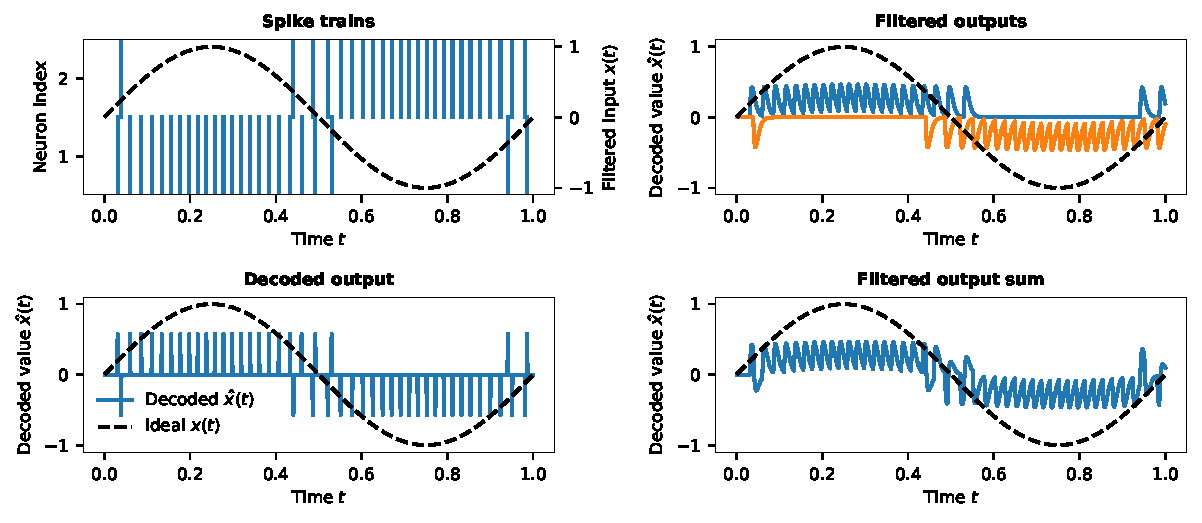
\includegraphics[width=\textwidth]{media/two_neurons_synaptic_filter.pdf}\\
	\centering $\tau = \SI{5}{\milli\second}, n = 1$
\end{frame}

\begin{frame}{Example: Synaptic Filter for One Hundred Neurons}
	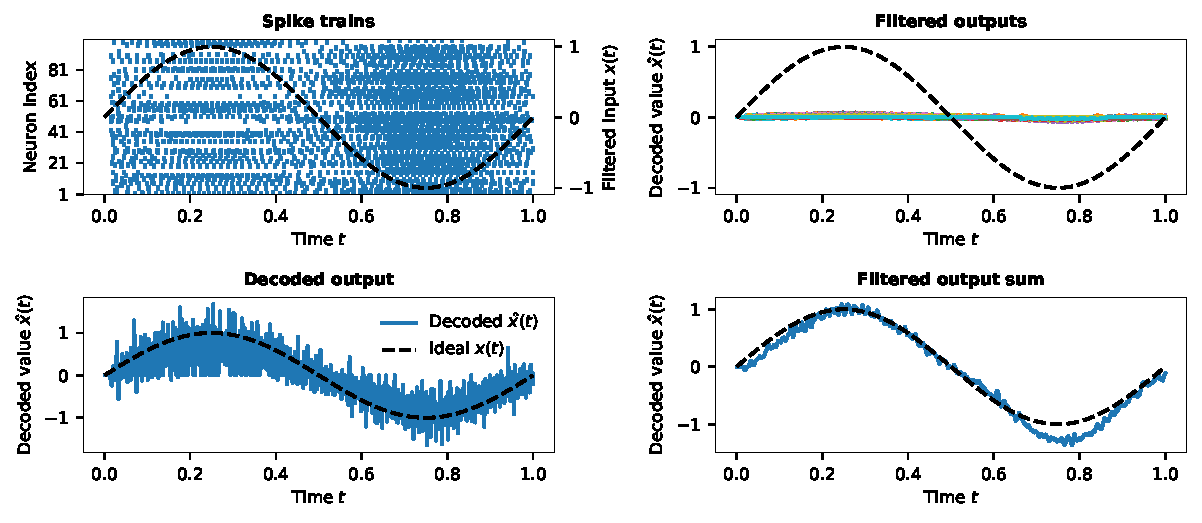
\includegraphics[width=\textwidth]{media/n_neurons_synaptic_filter.pdf}
	\centering $\tau = \SI{5}{\milli\second}, n = 1$
\end{frame}

\backupbegin

\begin{frame}[noframenumbering]{Image sources}
	\small
	\textbf{Title slide}\\\enquote{Captive balloon with clock face and bell, floating above the Eiffel Tower, Paris, France.}\\Author: Camille Grávis, between 1889 and 1900.\\From \href{https://commons.wikimedia.org/wiki/File:Camille_Gr\%C3\%A1vis,_Captive_balloon_with_clock_face_and_bell,_floating_above_the_Eiffel_Tower,_Paris,_France.jpg}{Wikimedia}.
\end{frame}


\backupend

\end{document}
